\documentclass[a4paper,12pt,oneside]{article}
\usepackage{amsmath,amssymb}
\usepackage{listings}
\usepackage{latexsym}
\usepackage{pdfpages}
\usepackage{graphicx}
\usepackage{url}
\usepackage[top=1in,bottom=1in,left=1.25in,right=1.25in]{geometry}
\bibliographystyle{ieeetr}
\title{GSoC'14:GSM Analysis Tool}
\date{\today}
\author{Zhenhua HAN\\ hzhua201@gmail.com\\ \\Mentor: Sylvain Munaut}


\begin{document}
\maketitle
\tableofcontents
\newpage
\section{Introduction}
GSM (Global System for Mobile Communications) is the most used standard in mobile communication. GNU Radio is a free software development toolkit that provides the signal processing runtime and processing blocks to implement software radios using readily-available, low-cost external RF hardware and commodity processors.\cite{gnuradio} This proposal addresses ideas to create an out of tree module for GNU Radio to decode GSM signals as suggested by Sylvain Munaut. Section 2 is the general description of the GSM physical layer as this project mainly focuses on decoding GSM signal. Section 3 is the deliverables. A rough project schedule is given in Section 4. My personal statements are in Section 5.
\section{Background of GSM Signal}
GSM (Global System for Mobile Communications) is a standard developed by the European Telecommunications Standards Institute (ETSI) to describe protocols for the second generation (2G) digital cellular networks used by mobile phones. According to the GSM Association, it is approximated that 80 percent of the world use GSM when placing wireless calls.

\subsection{Multiple access and time slot structure}
The access scheme of GSM is Time Division Multiple Access (TDMA) with 8 basic physical channels per carrier. The carriers are separated by 200kHz.

Figure \ref{fig:1} shows the time slot structure and bursts. The longest recurrent time period is called hyperframe which has a duration of 3h 28mn 53s 760ms. One hyperframe contains 2048 superframes which have a duration of 6.12 seconds. A superframe contains 26-frame multiframe (51 per superframe) or 51-frame multiframe(26 per superframe). One (26-frame) multiframe contains 26 TDMA frames and one (51-frame) multiframe contains 51 TDMA frames. A TDMA frame contains 8 time slots. A time slot is the basic radio resource of GSM which lasts about 576.9 $\mu s$ (15/26 ms) and 156.25 bit durations, and its physical content is called a burst. There are four types of bursts in GSM.

\begin{itemize}
\item normal burst (NB): This burst is used to carry information on traffic and control channels.
\item frequency correction burst (FB): This burst is used for frequency synchronization of the mobile.
\item synchronization burst (SB): This burst is used to time synchronization of the mobile.
\item access burst (AB): This burst is used for random access from a mobile which does not know the timing advance at the first access (or after the handover).
\end{itemize}

\newpage

\begin{figure}[!h]
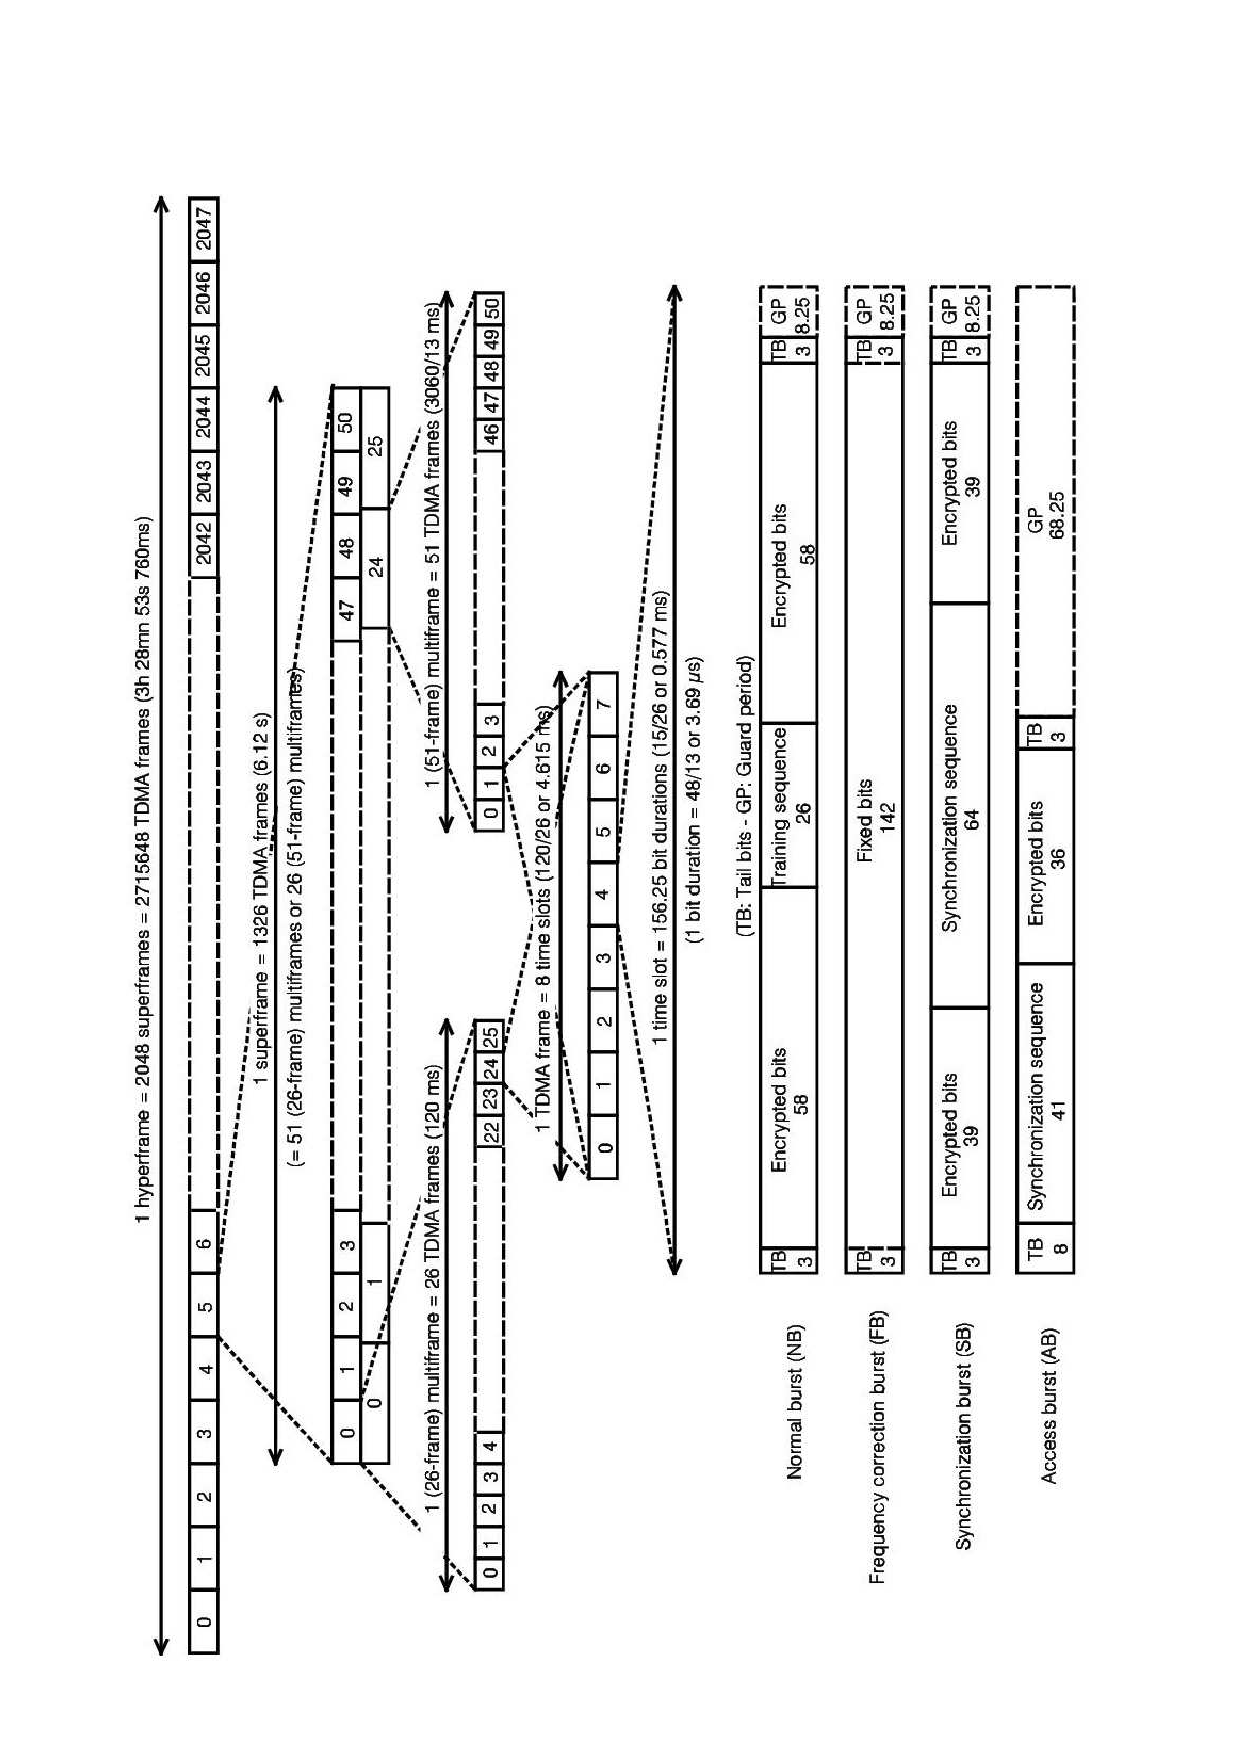
\includepdf{figure/timeframe.pdf}
\caption{Time frames, time slots and bursts \label{fig:1} \cite{etsi199203}}
\end{figure}
\newpage

\subsection{Channel organization}
In the GSM, there are two types of logical channels: Common Channels (CCH) and Dedicated Channels (DCH). As figure \ref{fig:2} shows, the CCH consists of Broadcasting Channels (BCH) and Common Control Channels (CCCH) and the DCH consists of Dedicated Control Channels (DCCH) and Traffic Channels (TCH). Figure \ref{fig:26f} and \ref{fig:51f} shows how the channel organized in the 26-frame multiframe and 51-frame multiframe respectively.

\begin{figure}[h]
\centering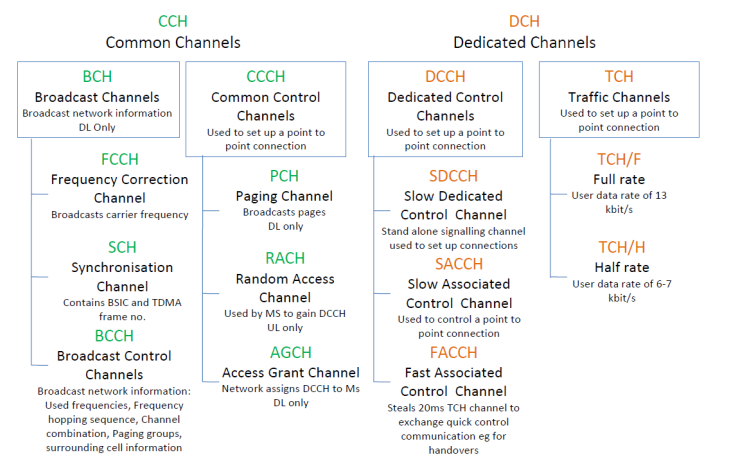
\includegraphics[width=5in]{figure/log_ch.png}
\caption{Logic Channels of GSM \label{fig:2} \cite{glendrange2010decoding}}
\end{figure}
\begin{figure}[h]
\centering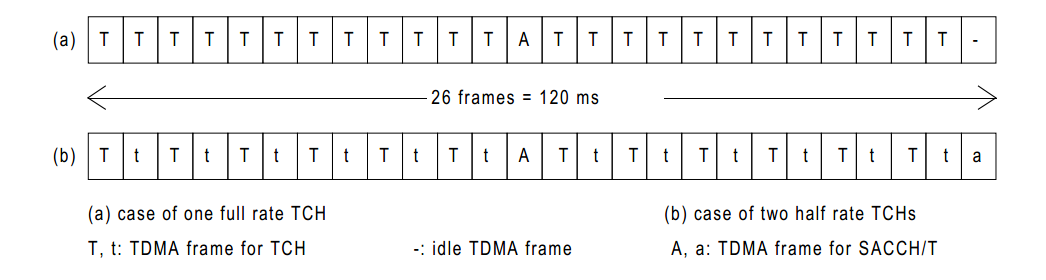
\includegraphics[width=5in]{figure/26frames.png}
\caption{ 26-frame organization\label{fig:26f} \cite{etsi199203}}
\end{figure}

\newpage
\begin{figure}[h]
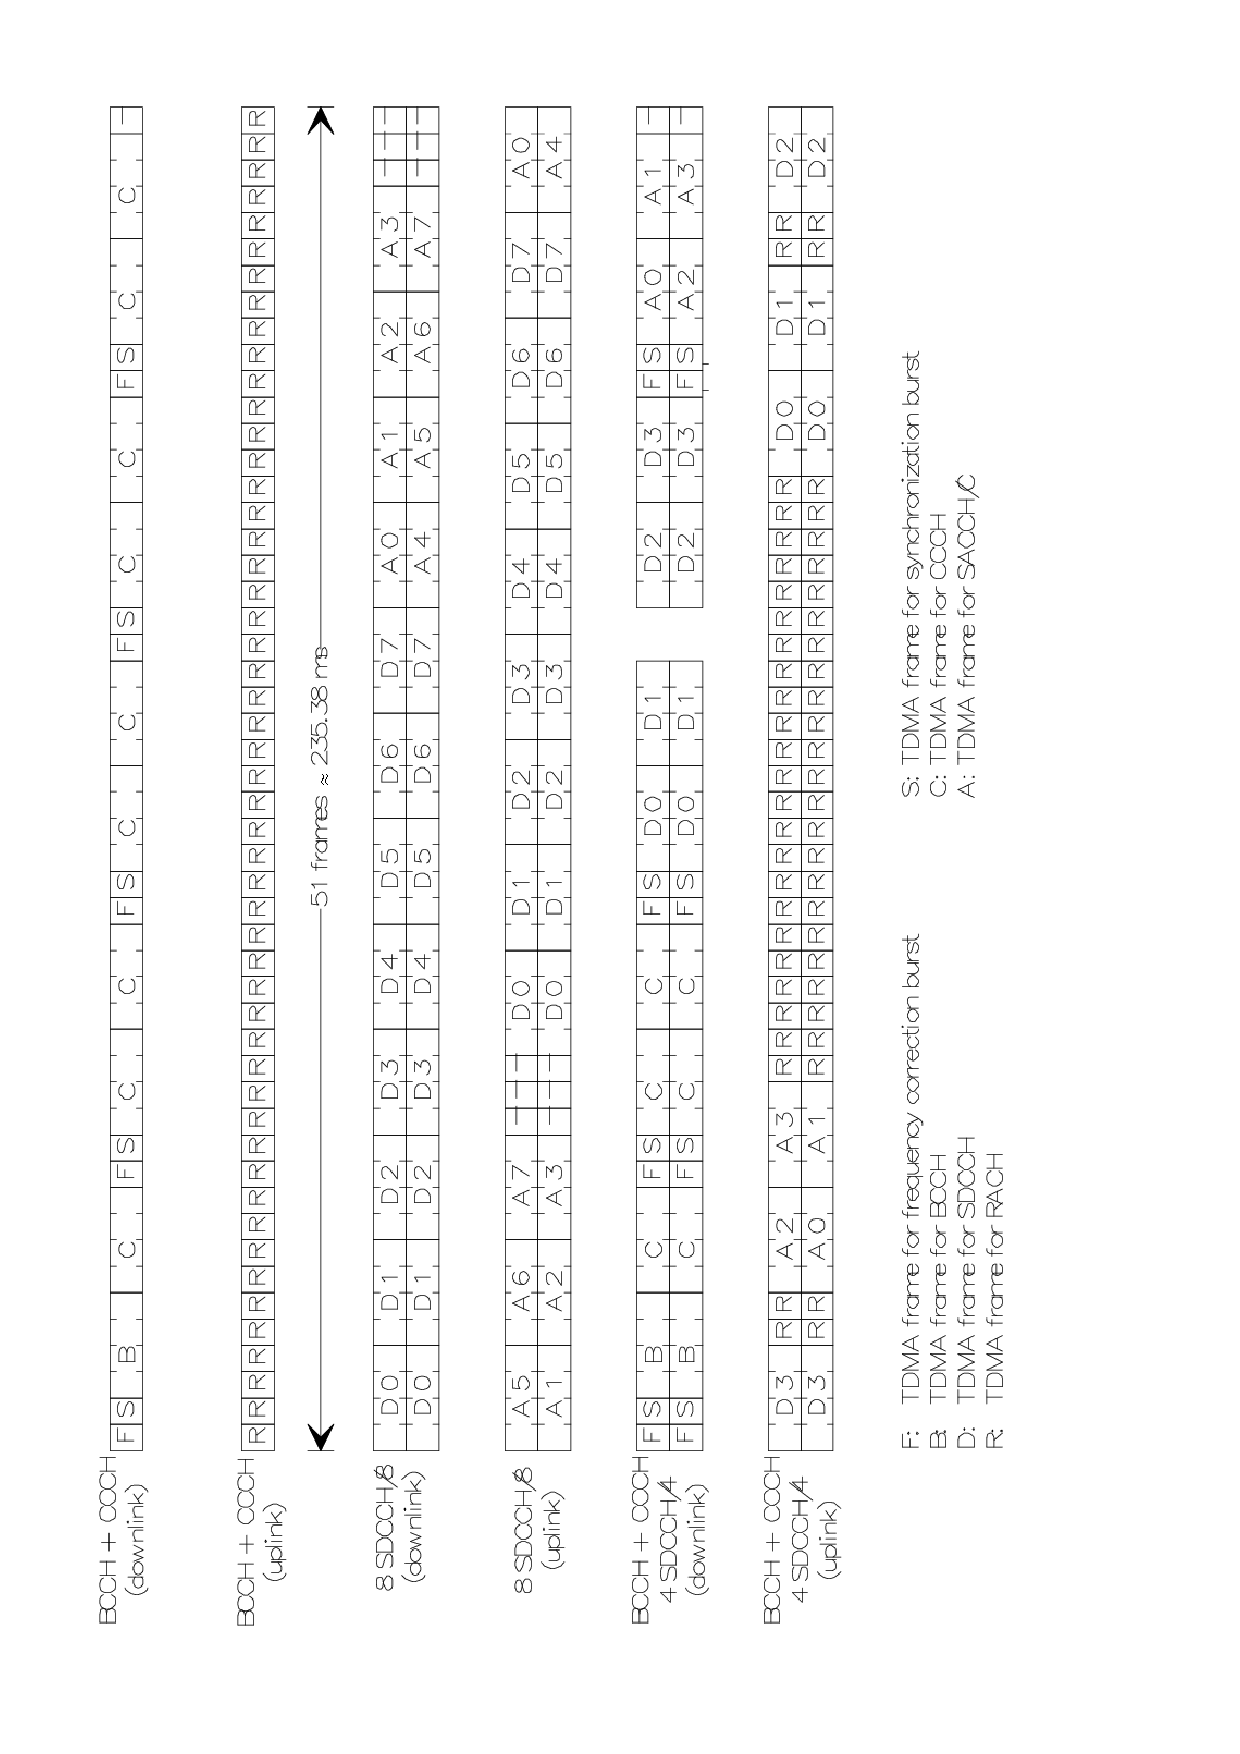
\includepdf[width=7in]{figure/51frames.pdf}
\caption{ 51-frame organization\label{fig:51f} \cite{etsi199203}}
\end{figure}

\newpage


\subsection{Coding schemes}
The table in figure \ref{fig:coding} shows the summarised description of the coding schemes of GSM. For all types of channels, the operations are made by the order of external coding(block coding), internal coding(convolutional coding) and then interleaving.

\begin{figure}[h]
\centering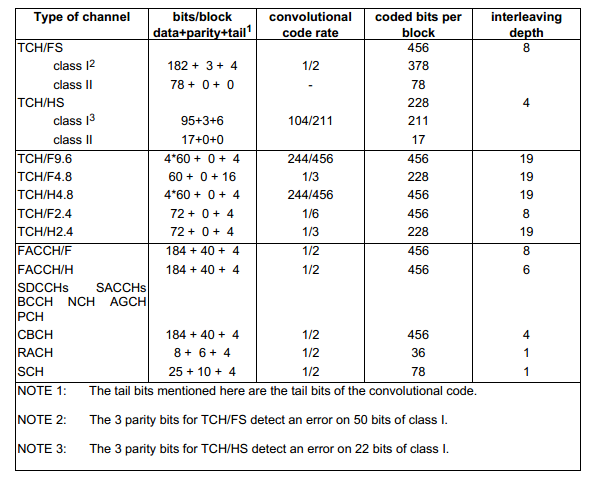
\includegraphics[width=5in]{figure/coding.png}
\caption{Channel block structure \label{fig:coding} \cite{etsi199203}}
\end{figure}


\section{Deliverables}
Airprobe is a tool that was used to analyse GSM signals a while back. It no longer works with current GNU Radio versions, and doesn't make use of any of the new GNU Radio features. A modular rewrite is the main part of this project. Figure \ref{fig:3} shows the blocks of GSM Analysis Tool which will be implemented in this project.


\begin{figure}[!h]
\centering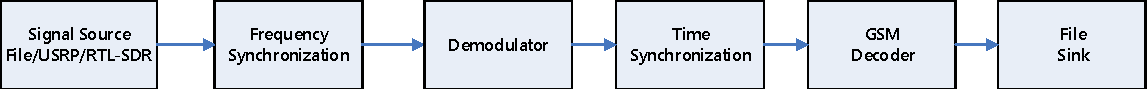
\includegraphics[width=5.4in]{figure/flowgraph.pdf}
\caption{Blocks of GSM Analysis Tool \label{fig:3}}
\end{figure}

\subsection{FCCH Burst Detection with adaptive filter}
Martin Braun (martin.braun@ettus.com) suggests a paper \cite{1404796} which introduced an algorithm for FCCH burst detection. The algorithm uses an adaptive filter to help distinguishing FCCH bursts from other bursts. I have implemented this algorithm for test and upload to my github : \url{https://github.com/hzhua/gr-fchdetection}.
As after GMSK modulation, the frequency correction bits is a sinusoid of frequency 67.7033KHz. The normal bursts at base-band are 100KHz.
Therefore, I used a FIR low pass filter with 70KHz pass band and 10KHz transition band. With the help of adaptive filter, it can detect
the FCCH burst fast and accurately. Figure \ref{fig:fch} shows the ratio of average error power to input power. The average error is very low
at frequency burst and high at other bursts. A threshold can be easily find to separate two parts.

\begin{figure}[!h]
\centering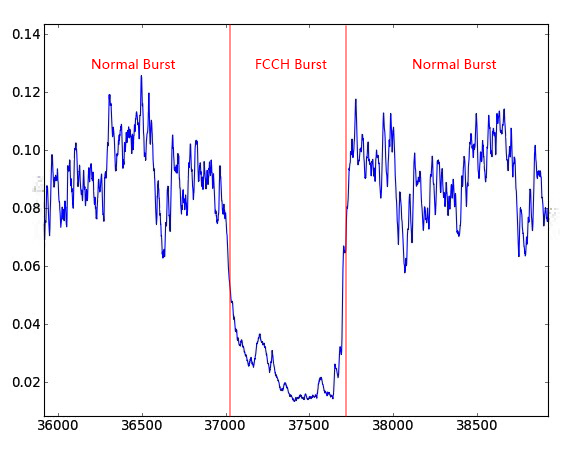
\includegraphics[width=5.4in]{figure/fcch_detect.png}
\caption{FCCH detected by an adaptive filter\label{fig:fch}}
\end{figure}


\subsection{Improving the performance of frequency correlation}

As Piot Krysik (perper@o2.pl) said, there is instability in the method of correction of the frequency offset in Airprobe. The reason is the lack of synchronization between computation of frequency offset and its correction inside of FIR filter. As Piot suggests, I will use stream tags to solve this problem.

\subsection{Using GNU Radio 3.7 new features}
\begin{itemize}
\item Correlate and Sync block is a new block added in GNU Radio 3.7.2. It is designed
to search for a preamble by correlation and uses the results of the
correlation to get a time and phase offset estimate.
It can be used to help GSM signal to get time synchronization.

\item The file sink in GNU Radio starts to support appending content into a file. This feature makes it easier to use with IPC.
As GSM Analysis Tool will support real-time decoding of GSM signal, it can be used to communicate with other tools for
further analysis.
\end{itemize}

\subsection{The Deliverables list}
\begin{itemize}
\item Deliverable 0: Create on out-of-tree module for GSM analysis tool (gr-gsm), using gr-modtool;
\item Deliverable 1: Get properly channelized / resampled data;
\item Deliverable 2: Find frequency correction burst (FB) and realize frequency synchronization;
\item Deliverable 3: Find synchronization burst (SB) and realize time synchronization;
\item Deliverable 4: Decode and decrypt the downlink of 26-frame multiframes for the traffic channel (TCH);
\item Deliverable 5: Decode and decrypt the downlink of 51-frame multiframes for 3 types of control channels ("BCCH+CCCH", "8SDCCH/8" and "BCCH+

    CCCH+4SDCCH/4");
\item Deliverable 6: Integrate all parts with real-time capabilities.
\end{itemize}

\section{Schedule}
As the schedule of GSoC'14 shows, there are 14 weeks including midterm evaluation and final evaluations. This schedule is a rough plan which may change after discussions with the mentor. The timeline is structured as follows:
\begin{itemize}
\item \textbf{1st Phase (2 weeks)} : Initial discussions with the mentor. Learn how to write an out-of-tree module of GNU Radio. Learn the detailed protocol of GSM.
\item \textbf{2nd Phase (1 week)} : OOT module is created. Data capturing is coded.
\item \textbf{3rd Phase (2 weeks)} : Frequency synchronization and GMSK demodulator with Viterbi algorithm is coded.
\item \textbf{4rd Phase (1 week)} : Start to code time synchronization.
\item \textbf{5th Phase (1 week)} : Mid-term evaluation and time synchronization is finished.
\item \textbf{6th Phase (2 weeks)} : TCH and Control Channel decoder is coded.
\item \textbf{7th Phase (3 weeks)} : Integrate all parts with real-time capabilities.
\item \textbf{8th Phase (2 weeks)} : QA test, code clean-up, adding documentation and final submission.

\end{itemize}
\section{Expanding tasks}
Because there is only 14 weeks in GSoC, it is too short to add other parts into this project during this 14 weeks. However I will keep improving gr-gsm after GSoC. Other expanding tasks will be added into gr-gsm after. Here is a list with part of them:

\begin{itemize}
\item frequency hopping protocol will be supported; (With high priority)
\item A physical layer of GSM transmitter will be added. With this transmitter, one can disguise himself into a cellphone or a base station.
\item GPRS will be supported;
\end{itemize}

\section{Qualification}
I'm a fourth year undergraduate in Electronic Information Engineering of University of Electronic Science and Technology of China. This fall, I will take up a PhD degree with a major in Computer Science in University of Hong Kong. I used to participate in the ACM International Collegiate Programming Contest (ICPC) and won two gold medals in Asia regional contest. My experience in ICPC greatly improved my algorithm and programming ability. Besides, I have been working on the research of Cognitive Radio Networks for a year. And I have submitted a paper on Cognitive Radio on WASA2014(The 9th International Conference on Wireless Algorithms, Systems, and Applications). \\

I got to know GNU Radio when I read a paper on cognitive radio which using GNU Radio and a USRP to analyse the algorithm in their paper. Then we bought a USRP to help our group in the research of cognitive radio. My easy access to USRP will help me in finishing the coding of GSM Analysis Tool.\\

On my coding experience, I was an intern in the Alibaba Group which is the biggest e-commerce company in China. I finished 60 percent codes of a Java project called Beacon. It uses Solr as searching engine to catch illegal users. My work was to optimize the searching engine and the coding of the back end. Unfortunately, the codes are under confidential. I also contributed my codes to an Open Source project SNSAPI (it is a Chinese project). You can find it in my github page: \url{https://github.com/hzhua/snsapi}.\\

As this is the biggest project I have dealt with, it may be a challenging task for me to complete in the given time span. If I cannot finish GSM Analysis Tool in 14 weeks, I will continue my works even after GSoC. For my personal motivation, I will continue my research on wireless networks during my PhD degree. Therefore I will use GNU Radio and USRP as powerful tools for many years. I would love to continue learning and working in GNU Radio community after GSoC. So, don't worry about if I will disappear during GSoC.\\

If you want to know me better, please visit my personal page \url{https//hzhua.github.io}. You can find my CV there.

I agree for my work to be published under the GPL license.

\section{Conclusion}
I hope I can win this chance to work in GNU Radio community. If you have any questions, don't be hesitated to contact me.
\bibliography{ref}

\end{document}
